% filepath: c:\REPO\studia\ZAAWANSOWANAOPTYMALIZACJA20252026\ProjektSieczne\main.tex
\documentclass[10pt,a4paper]{article}

% ...existing code...
% Kodowanie i język
\usepackage[utf8]{inputenc}
\usepackage[T1]{fontenc}
\usepackage[polish]{babel}

% Układ strony i mikrotypografia
\usepackage[a4paper,margin=15mm]{geometry}
\usepackage{lmodern}
\usepackage{microtype}

% Podstawowe pakiety
\usepackage{graphicx}
\usepackage{amsmath,amssymb}
\usepackage{siunitx}
\usepackage{booktabs}
\usepackage{caption}
\usepackage{hyperref}
\usepackage{algorithm}
\usepackage{algorithmic}
% \usepackage{algpseudocode}
\usepackage{float}
\usepackage{longtable}
\usepackage{booktabs}
\usepackage{minted}
\usepackage{listings}
\usepackage{xcolor}
\lstset{
  language=Matlab,
  basicstyle=\ttfamily\small,
  keywordstyle=\color{blue},
  commentstyle=\color{gray},
  frame=single,
  breaklines=true,
  numbers=left,
  numberstyle=\tiny,
  xleftmargin=1em
}


\hypersetup{colorlinks=true,linkcolor=blue,citecolor=blue,urlcolor=blue}

% Bibliografia (użyj biber lub zmień na natbib jeśli wolisz)
\usepackage[backend=biber,style=numeric,sorting=none]{biblatex}
\addbibresource{references.bib} % utwórz plik references.bib w katalogu projektu

% ...existing code...
\title{Metoda optymalizacji}
\author{Paweł Drzyzga \\ Wydział Informatyki i Matematyki \\ Politechnika Krakowska}
\date{\today}

\begin{document}
\maketitle


\tableofcontents
\clearpage

\section{Metody optymalizacji}

\subsection{Metoda Hooke’a--Jeevesa}

Metoda Hooke’a--Jeevesa jest bezgradientową, iteracyjną metodą optymalizacji,
przeznaczoną do wyznaczania minimum funkcji
\[
f:\mathbb{R}^2 \to \mathbb{R}.
\]
Algorytm opiera się wyłącznie na porównywaniu wartości funkcji w punktach
sąsiadujących z aktualnym przybliżeniem i nie wymaga obliczania pochodnych.

\subsubsection{Opis matematyczny algorytmu}

Niech $x^{(k)} = (x_1^{(k)}, x_2^{(k)})$ oznacza aktualny punkt w $k$-tej iteracji,
a $\delta > 0$ — aktualny krok przeszukiwania.
W algorytmie wykorzystywane są wektory bazowe przestrzeni $\mathbb{R}^2$:
\[
e_1 = (1,0), \qquad e_2 = (0,1).
\]

Jedna iteracja metody składa się z następujących etapów:

\begin{enumerate}
\item \textbf{Krok eksploracyjny.}
Dla każdej współrzędnej sprawdzane są punkty:
\[
x^{(k)} \pm \delta e_i, \quad i=1,2.
\]
Jeżeli w którymkolwiek z tych punktów wartość funkcji jest mniejsza niż
$f(x^{(k)})$, punkt zostaje zaktualizowany.

\item \textbf{Ruch wzorcowy.}
Jeżeli krok eksploracyjny zakończył się poprawą, wykonywany jest ruch wzorcowy:
\[
x_{\text{pattern}} = x_{\text{new}} + \alpha \bigl(x_{\text{new}} - x^{(k)}\bigr),
\]
gdzie $\alpha > 1$ jest ustalonym parametrem (w implementacji przyjęto $\alpha=2$).
Jeżeli $f(x_{\text{pattern}}) < f(x_{\text{new}})$, punkt wzorcowy zostaje zaakceptowany.

\item \textbf{Redukcja kroku.}
Jeżeli w kroku eksploracyjnym nie znaleziono poprawy, krok jest zmniejszany:
\[
\delta \leftarrow \frac{\delta}{2}.
\]
\end{enumerate}

Algorytm jest wykonywany iteracyjnie aż do spełnienia kryterium stopu:
\[
\delta \le \varepsilon,
\]
gdzie $\varepsilon > 0$ jest zadaną tolerancją.



\subsubsection{Przykład liczbowy}

Rozważmy funkcję:
\[
f(x,y) = (x-1)^2 + (y-2)^2,
\]
która posiada minimum globalne w punkcie $(1,2)$.

Dane początkowe:
\[
x^{(0)} = (4,4), \quad \delta_0 = 2, \quad \alpha = 2, \quad \varepsilon = 0.5.
\]

Wartość funkcji w punkcie startowym:
\[
f(4,4) = (4-1)^2 + (4-2)^2 = 13.
\]

\paragraph{Iteracja 1.}

\emph{Krok eksploracyjny w kierunku osi $x$:}
\[
f(6,4) = 29, \qquad f(2,4) = 5.
\]
Punkt zostaje zaktualizowany do $(2,4)$.

\emph{Krok eksploracyjny w kierunku osi $y$:}
\[
f(2,6) = 17, \qquad f(2,2) = 1.
\]
Nowy punkt:
\[
x^{(1)} = (2,2).
\]

\emph{Ruch wzorcowy:}
\[
x_{\text{pattern}} = (2,2) + 2\big((2,2)-(4,4)\big) = (-2,-2),
\]
\[
f(-2,-2) = 25.
\]
Ruch wzorcowy zostaje odrzucony.



\paragraph{Iteracja 2.}

Dla $\delta = 2$ sprawdzane punkty:
\[
(4,2),\ (0,2),\ (2,4),\ (2,0),
\]
nie dają poprawy wartości funkcji.
W związku z tym krok zostaje zredukowany:
\[
\delta \leftarrow 1.
\]



\paragraph{Iteracja 3.}

\emph{Krok eksploracyjny w kierunku osi $x$:}
\[
f(3,2) = 4, \qquad f(1,2) = 0.
\]
Punkt zostaje zaktualizowany do $(1,2)$.

\emph{Krok eksploracyjny w kierunku osi $y$:}
\[
f(1,3) = 1, \qquad f(1,1) = 1.
\]
Brak dalszej poprawy.



\subsubsection{Wynik końcowy}

Po trzech iteracjach algorytmu otrzymano punkt:
\[
x^* = (1,2),
\]
który jest minimum globalnym analizowanej funkcji.



\subsubsection{Pseudokod}

\begin{algorithm}[H]
\caption{Metoda poszukiwań wzorcowych (Hooke--Jeeves)}
\begin{algorithmic}[1]
\STATE \textbf{Dane:} funkcja $f(x)$, punkt startowy $x_0$, krok początkowy $\delta_0$, tolerancja $\varepsilon$
\STATE \textbf{Wynik:} przybliżone minimum $x^\ast$

\STATE $x \leftarrow x_0$
\STATE $\delta \leftarrow \delta_0$

\WHILE{$\delta > \varepsilon$}
    \STATE $x_{\text{new}} \leftarrow x$
    \FOR{każda współrzędna $i$}
        \IF{$f(x_{\text{new}} + \delta e_i) < f(x_{\text{new}})$}
            \STATE $x_{\text{new}} \leftarrow x_{\text{new}} + \delta e_i$
        \ELSIF{$f(x_{\text{new}} - \delta e_i) < f(x_{\text{new}})$}
            \STATE $x_{\text{new}} \leftarrow x_{\text{new}} - \delta e_i$
        \ENDIF
    \ENDFOR

    \IF{$f(x_{\text{new}}) < f(x)$}
        \STATE $x \leftarrow x + (x_{\text{new}} - x)$ \COMMENT{ruch wzorcowy}
    \ELSE
        \STATE $\delta \leftarrow \delta / 2$
    \ENDIF
\ENDWHILE

\STATE $x^\ast \leftarrow x$
\end{algorithmic}
\end{algorithm}



\subsubsection{Uwagi końcowe}

Metoda Hooke’a--Jeevesa wykorzystuje wyłącznie porównania wartości funkcji
oraz proste operacje arytmetyczne. Dzięki temu jest odporna na brak gładkości
funkcji, jednak jej zbieżność może być wolniejsza w porównaniu z metodami
gradientowymi.

\subsection{Metoda Neldera--Meada (simpleks)}

Metoda Neldera--Meada jest bezgradientową, iteracyjną metodą optymalizacji
przeznaczoną do minimalizacji funkcji
\[
f:\mathbb{R}^2 \to \mathbb{R}.
\]
Algorytm nie operuje na pojedynczym punkcie, lecz na zbiorze punktów tworzących
\emph{simpleks}. W przestrzeni dwuwymiarowej simpleks składa się z trzech
wierzchołków.

Metoda wykorzystuje jedynie wartości funkcji w wierzchołkach simpleksu oraz
proste operacje liniowe na wektorach, bez konieczności obliczania pochodnych.



\subsubsection{Opis matematyczny algorytmu}

Niech
\[
S^{(k)} = \{x_1^{(k)}, x_2^{(k)}, x_3^{(k)}\}
\]
oznacza simpleks w $k$-tej iteracji. W każdej iteracji wierzchołki są sortowane
według wartości funkcji:
\[
f(x_B^{(k)}) \le f(x_G^{(k)}) \le f(x_W^{(k)}),
\]
gdzie:
\begin{itemize}
\item $x_B^{(k)}$ — najlepszy punkt,
\item $x_G^{(k)}$ — punkt pośredni,
\item $x_W^{(k)}$ — najgorszy punkt.
\end{itemize}

Centroid simpleksu (z pominięciem najgorszego punktu) dany jest wzorem:
\[
c^{(k)} = \frac{1}{2}\bigl(x_B^{(k)} + x_G^{(k)}\bigr).
\]

Na tej podstawie wyznaczane są kolejne punkty testowe:

\begin{itemize}
\item \textbf{Odbicie}:
\[
x_R = c^{(k)} + \alpha\bigl(c^{(k)} - x_W^{(k)}\bigr),
\]
\item \textbf{Ekspansja}:
\[
x_E = c^{(k)} + \gamma\bigl(x_R - c^{(k)}\bigr),
\]
\item \textbf{Kontrakcja}:
\[
x_C = c^{(k)} + \tfrac{1}{2}\bigl(x_W^{(k)} - c^{(k)}\bigr),
\]
\end{itemize}

gdzie $\alpha>0$ oraz $\gamma>1$ są ustalonymi parametrami algorytmu
(w implementacji przyjęto $\alpha=1$, $\gamma=2$).

W zależności od wartości funkcji w punktach $x_R$, $x_E$ oraz $x_C$,
najgorszy wierzchołek simpleksu zostaje zastąpiony odpowiednim punktem.



\subsubsection{Przykład liczbowy}

Rozważmy funkcję:
\[
f(x,y) = (x-1)^2 + (y-2)^2,
\]
która posiada minimum globalne w punkcie $(1,2)$.

Jako simpleks początkowy przyjmujemy:
\[
x_1^{(0)}=(4,4), \quad
x_2^{(0)}=(6,4), \quad
x_3^{(0)}=(4,6).
\]

Wartości funkcji:
\[
f(4,4)=13, \quad f(6,4)=29, \quad f(4,6)=25.
\]



\paragraph{Iteracja 1.}

Po posortowaniu wierzchołków:
\[
x_B=(4,4), \quad x_G=(4,6), \quad x_W=(6,4).
\]

Centroid:
\[
c = \frac{(4,4)+(4,6)}{2} = (4,5).
\]

Odbicie:
\[
x_R = 2c - x_W = (2,6),
\quad f(2,6)=17.
\]

Ponieważ $f(x_B) < f(x_R) < f(x_G)$, punkt $x_R$ zostaje zaakceptowany
i zastępuje $x_W$.

Nowy simpleks:
\[
(4,4),\ (4,6),\ (2,6).
\]



\paragraph{Iteracja 2.}

Po sortowaniu:
\[
x_B=(4,4), \quad x_G=(2,6), \quad x_W=(4,6).
\]

Centroid:
\[
c = \frac{(4,4)+(2,6)}{2} = (3,5).
\]

Odbicie:
\[
x_R = 2c - x_W = (2,4),
\quad f(2,4)=5.
\]

Ponieważ $f(x_R) < f(x_B)$, wykonywana jest ekspansja:
\[
x_E = c + 2(x_R - c) = (1,3),
\quad f(1,3)=1.
\]

Punkt $x_E$ zostaje zaakceptowany.



\paragraph{Iteracja 3.}

Simpleks:
\[
(4,4),\ (2,6),\ (1,3).
\]

Po dalszych operacjach odbicia i kontrakcji simpleks ulega stopniowemu
zmniejszeniu i koncentruje się w otoczeniu punktu $(1,2)$.



\subsubsection{Kryterium zakończenia}

Algorytm Neldera--Meada kończy działanie, gdy spełnione jest jedno z kryteriów:
\begin{itemize}
\item rozmiar simpleksu jest mniejszy od zadanej tolerancji,
\item różnice wartości funkcji w wierzchołkach simpleksu są niewielkie,
\item osiągnięto maksymalną liczbę iteracji.
\end{itemize}



\subsubsection{Wynik końcowy}

W zaprezentowanym przykładzie algorytm zbiega do punktu:
\[
x^* \approx (1,2),
\]
który jest minimum globalnym analizowanej funkcji.



\subsubsection{Pseudokod}

\begin{algorithm}[H]
\caption{Metoda Neldera--Meada (simpleksowa)}
\begin{algorithmic}[1]
\STATE \textbf{Dane:} funkcja $f(x)$, punkt startowy $x_0$, tolerancja $\varepsilon$
\STATE \textbf{Wynik:} minimum $x^\ast$
\STATE Zainicjalizuj simpleks $\{x_1, x_2, x_3\}$

\WHILE{kryterium stopu nie jest spełnione}
    \STATE Posortuj wierzchołki simpleksu według wartości $f$
    \STATE Wyznacz $x_{\text{best}},\, x_{\text{second\_worst}},\, x_{\text{worst}}$
    \STATE Wyznacz środek ciężkości $c$ bez najgorszego punktu:
    \STATE \hspace{0.5cm} $c \leftarrow \dfrac{1}{2}\left(x_{\text{best}} + x_{\text{second\_worst}}\right)$

    \STATE \textbf{Odbicie:} $x_r \leftarrow c + \alpha\left(c - x_{\text{worst}}\right)$
    \IF{$f(x_{\text{best}}) \le f(x_r)$ \AND $f(x_r) < f(x_{\text{second\_worst}})$}
        \STATE Zastąp $x_{\text{worst}} \leftarrow x_r$
    \ELSE
        \IF{$f(x_r) < f(x_{\text{best}})$}
            \STATE \textbf{Ekspansja:} $x_e \leftarrow c + \gamma\left(x_r - c\right)$
            \IF{$f(x_e) < f(x_r)$}
                \STATE Zastąp $x_{\text{worst}} \leftarrow x_e$
            \ELSE
                \STATE Zastąp $x_{\text{worst}} \leftarrow x_r$
            \ENDIF
        \ELSE
            \STATE Wykonaj \textbf{kontrakcję} albo \textbf{redukcję} simpleksu
        \ENDIF
    \ENDIF
\ENDWHILE

\STATE $x^\ast \leftarrow x_{\text{best}}$
\end{algorithmic}
\end{algorithm}


\subsubsection{Uwagi końcowe}

Metoda Neldera--Meada jest szczególnie użyteczna w przypadku funkcji,
dla których obliczanie pochodnych jest trudne lub niemożliwe. Jej wadą
jest brak gwarancji zbieżności do minimum globalnego w przypadku funkcji
o złożonej strukturze.


\subsection{Metoda Powella}

Metoda Powella jest bezgradientową, iteracyjną metodą optymalizacji,
przeznaczoną do minimalizacji funkcji
\[
f:\mathbb{R}^2 \to \mathbb{R}.
\]
Algorytm polega na wykonywaniu kolejnych minimalizacji jednowymiarowych
wzdłuż zadanych kierunków, które są aktualizowane w trakcie działania
algorytmu. Metoda nie wymaga obliczania pochodnych funkcji.



\subsubsection{Opis matematyczny algorytmu}

Niech $x^{(k)} \in \mathbb{R}^2$ oznacza punkt w $k$-tej iteracji algorytmu,
a zbiór kierunków:
\[
D^{(k)} = \{ d_1^{(k)}, d_2^{(k)} \}
\]
stanowi bazę kierunków przeszukiwania.

Początkowo przyjmuje się:
\[
d_1^{(0)} = (1,0), \qquad d_2^{(0)} = (0,1).
\]

Jedna iteracja metody Powella składa się z następujących etapów:

\begin{enumerate}
\item \textbf{Minimalizacja wzdłuż kierunku $d_1^{(k)}$:}
\[
x \leftarrow \arg\min_{\alpha} f\bigl(x^{(k)} + \alpha d_1^{(k)}\bigr).
\]

\item \textbf{Minimalizacja wzdłuż kierunku $d_2^{(k)}$:}
\[
x \leftarrow \arg\min_{\alpha} f(x + \alpha d_2^{(k)}).
\]

\item \textbf{Wyznaczenie nowego kierunku:}
\[
d_{\text{new}} = x - x^{(k)}.
\]

\item \textbf{Aktualizacja zbioru kierunków:}
\[
D^{(k+1)} = \{ d_2^{(k)}, d_{\text{new}} \}.
\]
\end{enumerate}

Algorytm jest wykonywany iteracyjnie aż do spełnienia kryterium stopu:
\[
\|x^{(k+1)} - x^{(k)}\| < \varepsilon,
\]
gdzie $\varepsilon > 0$ jest zadaną tolerancją.



\subsubsection{Przykład liczbowy}

Rozważmy funkcję:
\[
f(x,y) = (x-1)^2 + (y-2)^2,
\]
która posiada minimum globalne w punkcie $(1,2)$.

Dane początkowe:
\[
x^{(0)} = (4,4),
\quad
d_1^{(0)} = (1,0),
\quad
d_2^{(0)} = (0,1).
\]



\paragraph{Iteracja 1.}

\emph{Minimalizacja wzdłuż kierunku $d_1^{(0)}=(1,0)$:}

Rozważamy funkcję jednej zmiennej:
\[
\varphi_1(\alpha) = f(4+\alpha, 4)
= (3+\alpha)^2 + 4.
\]

Minimum osiągane jest dla:
\[
\alpha^* = -3.
\]

Nowy punkt:
\[
x = (4,4) + (-3)(1,0) = (1,4).
\]



\emph{Minimalizacja wzdłuż kierunku $d_2^{(0)}=(0,1)$:}

\[
\varphi_2(\alpha) = f(1,4+\alpha)
= (2+\alpha)^2.
\]

Minimum osiągane jest dla:
\[
\alpha^* = -2.
\]

Nowy punkt:
\[
x^{(1)} = (1,2).
\]



\emph{Wyznaczenie nowego kierunku:}
\[
d_{\text{new}} = x^{(1)} - x^{(0)} = (-3,-2).
\]

Zaktualizowany zbiór kierunków:
\[
d_1^{(1)} = (0,1), \qquad d_2^{(1)} = (-3,-2).
\]



\paragraph{Iteracja 2.}

\emph{Minimalizacja wzdłuż kierunku $d_1^{(1)}=(0,1)$:}

\[
\varphi_1(\alpha) = f(1,2+\alpha) = \alpha^2,
\]
co prowadzi do minimum dla $\alpha = 0$.



\emph{Minimalizacja wzdłuż kierunku $d_2^{(1)}=(-3,-2)$:}

\[
\varphi_2(\alpha) = f(1-3\alpha, 2-2\alpha)
= 13\alpha^2,
\]
której minimum również osiągane jest dla $\alpha = 0$.

Ponieważ punkt nie ulega zmianie, algorytm spełnia kryterium stopu.



\subsubsection{Wynik końcowy}

Metoda Powella zakończyła działanie po dwóch iteracjach,
zwracając punkt:
\[
x^* = (1,2),
\]
który jest minimum globalnym analizowanej funkcji.



\subsubsection{Pseudokod}

\begin{algorithm}[H]
\caption{Metoda Powella (bezpochodna, z przeszukiwaniem liniowym)}
\begin{algorithmic}[1]
\STATE \textbf{Dane:} funkcja $f(x)$, punkt startowy $x_0$, tolerancja $\varepsilon$
\STATE \textbf{Wynik:} minimum $x^\ast$

\STATE Ustal zbiór kierunków $D = \{e_1, e_2\}$
\STATE $x \leftarrow x_0$

\WHILE{nie spełniono kryterium stopu}
    \STATE $x_{\text{start}} \leftarrow x$

    \FOR{każdy kierunek $d \in D$}
        \STATE Wyznacz
        \STATE \hspace{0.5cm} $\alpha^\ast \leftarrow \arg\min_{\alpha} f(x + \alpha d)$
        \STATE $x \leftarrow x + \alpha^\ast d$
    \ENDFOR

    \STATE $d_{\text{new}} \leftarrow x - x_{\text{start}}$
    \STATE Zastąp jeden z kierunków w $D$ przez $d_{\text{new}}$
\ENDWHILE

\STATE $x^\ast \leftarrow x$
\end{algorithmic}
\end{algorithm}


\subsubsection{Uwagi końcowe}

Metoda Powella jest skuteczna w przypadku funkcji gładkich i
niskowymiarowych. Jej zaletą jest brak konieczności obliczania
gradientów, natomiast wadą może być szybki wzrost kosztu obliczeń
dla funkcji o wyższym wymiarze.

\subsection{Metoda Fletcher--Reevesa}

Metoda Fletcher--Reevesa należy do klasy gradientowych metod iteracyjnych
i stanowi wariant metody sprzężonych gradientów.
Jej celem jest minimalizacja funkcji
\[
f:\mathbb{R}^2 \to \mathbb{R},
\]
przy wykorzystaniu informacji o gradiencie funkcji oraz kierunków
sprzężonych, które zapewniają szybszą zbieżność niż metoda najszybszego
spadku.



\subsubsection{Opis matematyczny algorytmu}

Niech $x^{(k)} \in \mathbb{R}^2$ oznacza punkt w $k$-tej iteracji algorytmu,
a gradient funkcji w tym punkcie:
\[
g^{(k)} = \nabla f(x^{(k)}).
\]

Kierunek poszukiwań definiowany jest jako:
\[
d^{(k)} =
\begin{cases}
- g^{(0)}, & k = 0,\\[6pt]
- g^{(k)} + \beta_k d^{(k-1)}, & k \ge 1,
\end{cases}
\]
gdzie współczynnik Fletcher--Reevesa dany jest wzorem:
\[
\beta_k =
\frac{\|g^{(k)}\|^2}{\|g^{(k-1)}\|^2}.
\]

Aktualizacja punktu następuje zgodnie z zależnością:
\[
x^{(k+1)} = x^{(k)} + \alpha_k d^{(k)},
\]
gdzie $\alpha_k > 0$ jest krokiem wyznaczanym w procesie
jednowymiarowej minimalizacji wzdłuż kierunku $d^{(k)}$.

Algorytm jest powtarzany aż do spełnienia kryterium stopu:
\[
\|\nabla f(x^{(k)})\| < \varepsilon.
\]



\subsubsection{Przykład liczbowy}

Rozważmy funkcję:
\[
f(x,y) = x^2 + 2y^2,
\]
która posiada minimum globalne w punkcie $(0,0)$.

Gradient funkcji:
\[
\nabla f(x,y) = (2x, 4y).
\]

Dane początkowe:
\[
x^{(0)} = (1,1), \qquad \varepsilon > 0.
\]



\paragraph{Iteracja 0.}

Gradient:
\[
g^{(0)} = (2,4).
\]

Kierunek:
\[
d^{(0)} = -g^{(0)} = (-2,-4).
\]

Rozważamy funkcję jednej zmiennej:
\[
\varphi(\alpha) = f(1-2\alpha, 1-4\alpha)
= 3 - 20\alpha + 36\alpha^2.
\]

Minimum osiągane jest dla:
\[
\alpha_0 = \frac{5}{18}.
\]

Nowy punkt:
\[
x^{(1)} =
(1,1) + \frac{5}{18}(-2,-4)
=
\left(\frac{4}{9}, -\frac{1}{9}\right).
\]



\paragraph{Iteracja 1.}

Gradient:
\[
g^{(1)} =
\left(\frac{8}{9}, -\frac{4}{9}\right).
\]

Współczynnik:
\[
\beta_1 =
\frac{\|g^{(1)}\|^2}{\|g^{(0)}\|^2}
=
\frac{80/81}{20}
=
\frac{4}{81}.
\]

Kierunek:
\[
d^{(1)} =
- g^{(1)} + \beta_1 d^{(0)}
=
\left(-\frac{80}{81}, \frac{20}{81}\right).
\]

Po wykonaniu line search otrzymujemy:
\[
\alpha_1 = \frac{9}{20}.
\]

Nowy punkt:
\[
x^{(2)} =
\left(\frac{4}{9}, -\frac{1}{9}\right)
+
\frac{9}{20}
\left(-\frac{80}{81}, \frac{20}{81}\right)
=
(0,0).
\]



\paragraph{Iteracja 2.}

Gradient:
\[
g^{(2)} = (0,0).
\]

Ponieważ $\|\nabla f(x^{(2)})\| = 0$, spełnione jest kryterium stopu
i algorytm zostaje zakończony.



\subsubsection{Wynik końcowy}

Metoda Fletcher--Reevesa zakończyła działanie po trzech iteracjach,
zwracając punkt:
\[
x^* = (0,0),
\]
który jest minimum globalnym analizowanej funkcji.



\subsubsection{Pseudokod}

\begin{algorithm}[H]
\caption{Metoda gradientów sprzężonych (Fletchera--Reevesa)}
\begin{algorithmic}[1]
\STATE \textbf{Dane:} funkcja $f(x)$, punkt startowy $x_0$, tolerancja $\varepsilon$
\STATE \textbf{Wynik:} minimum $x^\ast$

\STATE $x \leftarrow x_0$
\STATE $g \leftarrow \nabla f(x)$
\STATE $d \leftarrow -g$

\WHILE{$\|g\| > \varepsilon$}
    \STATE Wyznacz krok $\alpha$ (przeszukiwanie liniowe)
    \STATE $x_{\text{new}} \leftarrow x + \alpha d$
    \STATE $g_{\text{new}} \leftarrow \nabla f(x_{\text{new}})$

    \STATE $\beta \leftarrow \dfrac{g_{\text{new}}^{T} g_{\text{new}}}{g^{T} g}$
    \STATE $d \leftarrow -g_{\text{new}} + \beta d$

    \STATE $x \leftarrow x_{\text{new}}$
    \STATE $g \leftarrow g_{\text{new}}$
\ENDWHILE

\STATE $x^\ast \leftarrow x$
\end{algorithmic}
\end{algorithm}


\subsubsection{Uwagi końcowe}

Metoda Fletcher--Reevesa wykorzystuje informację o gradiencie funkcji
oraz sprzężone kierunki poszukiwań, co pozwala na szybszą zbieżność
w porównaniu z metodą najszybszego spadku. Dla funkcji kwadratowych
algorytm osiąga minimum w skończonej liczbie iteracji.


\subsection{Metoda DFP (Davidon--Fletcher--Powell)}

Metoda DFP należy do klasy metod quasi-Newtona i służy do minimalizacji
funkcji
\[
f:\mathbb{R}^2 \to \mathbb{R}
\]
z wykorzystaniem informacji o gradiencie, bez konieczności jawnego
obliczania macierzy Hesjana. Algorytm konstruuje w kolejnych iteracjach
aproksymację odwrotności Hesjana, co pozwala na szybszą zbieżność niż
w klasycznych metodach gradientowych.



\subsubsection{Opis matematyczny algorytmu}

Niech $x^{(k)} \in \mathbb{R}^2$ oznacza punkt w $k$-tej iteracji algorytmu,
a gradient funkcji w tym punkcie:
\[
g^{(k)} = \nabla f(x^{(k)}).
\]

W metodzie DFP przechowywana jest macierz $H_k$, stanowiąca przybliżenie
odwrotności Hesjana $\bigl(\nabla^2 f(x^{(k)})\bigr)^{-1}$.
Kierunek poszukiwań wyznaczany jest jako:
\[
d^{(k)} = - H_k g^{(k)}.
\]

Po wykonaniu jednowymiarowej minimalizacji wzdłuż kierunku $d^{(k)}$
otrzymuje się nowy punkt:
\[
x^{(k+1)} = x^{(k)} + \alpha_k d^{(k)}.
\]

Definiujemy wektory:
\[
s_k = x^{(k+1)} - x^{(k)}, \qquad
y_k = g^{(k+1)} - g^{(k)}.
\]

Aktualizacja macierzy $H_k$ w metodzie DFP dana jest wzorem:
\[
H_{k+1}
=
H_k
+
\frac{s_k s_k^{\mathsf T}}{s_k^{\mathsf T} y_k}
-
\frac{H_k y_k y_k^{\mathsf T} H_k}{y_k^{\mathsf T} H_k y_k}.
\]

Algorytm jest wykonywany iteracyjnie aż do spełnienia kryterium stopu:
\[
\|\nabla f(x^{(k)})\| < \varepsilon.
\]



\subsubsection{Przykład liczbowy}

Rozważmy funkcję:
\[
f(x,y) = x^2 + 2y^2,
\]
która posiada minimum globalne w punkcie $(0,0)$.

Gradient funkcji:
\[
\nabla f(x,y) = (2x, 4y).
\]

Dane początkowe:
\[
x^{(0)} = (1,1), \qquad
H_0 =
\begin{pmatrix}
1 & 0\\
0 & 1
\end{pmatrix}.
\]



\paragraph{Iteracja 0.}

Gradient:
\[
g^{(0)} = (2,4).
\]

Kierunek:
\[
d^{(0)} = -H_0 g^{(0)} = (-2,-4).
\]

Jednowymiarowa minimalizacja prowadzi do kroku:
\[
\alpha_0 = \frac{5}{18}.
\]

Nowy punkt:
\[
x^{(1)} =
(1,1) + \frac{5}{18}(-2,-4)
=
\left(\frac{4}{9}, -\frac{1}{9}\right).
\]

Gradient:
\[
g^{(1)} =
\left(\frac{8}{9}, -\frac{4}{9}\right).
\]



\paragraph{Aktualizacja macierzy $H_1$.}

\[
s_0 =
\left(-\frac{5}{9}, -\frac{10}{9}\right), \qquad
y_0 =
\left(-\frac{10}{9}, -\frac{40}{9}\right).
\]

Po podstawieniu do wzoru DFP otrzymujemy nową macierz $H_1$, która
lepiej aproksymuje odwrotność Hesjana funkcji $f$.



\paragraph{Iteracja 1.}

Kierunek:
\[
d^{(1)} = -H_1 g^{(1)}.
\]

Po wykonaniu jednowymiarowej minimalizacji wzdłuż tego kierunku
otrzymujemy punkt:
\[
x^{(2)} = (0,0).
\]

Gradient:
\[
g^{(2)} = (0,0).
\]

Ponieważ $\|\nabla f(x^{(2)})\| = 0$, spełnione jest kryterium stopu
i algorytm zostaje zakończony.



\subsubsection{Wynik końcowy}

Metoda DFP zakończyła działanie po dwóch iteracjach,
zwracając punkt:
\[
x^\ast = (0,0),
\]
który jest minimum globalnym analizowanej funkcji.


\subsubsection{Pseudokod}

\begin{algorithm}[H]
\caption{Metoda BFGS (quasi-Newtona)}
\begin{algorithmic}[1]
\STATE \textbf{Dane:} funkcja $f(x)$, punkt startowy $x_0$, tolerancja $\varepsilon$
\STATE \textbf{Wynik:} minimum $x^\ast$

\STATE $x \leftarrow x_0$
\STATE $H \leftarrow I$ \COMMENT{początkowa aproksymacja odwrotności Hesjanu}

\WHILE{$\|\nabla f(x)\| > \varepsilon$}
    \STATE $d \leftarrow - H \nabla f(x)$
    \STATE Wyznacz krok $\alpha$ (przeszukiwanie liniowe)
    \STATE $x_{\text{new}} \leftarrow x + \alpha d$

    \STATE $s \leftarrow x_{\text{new}} - x$
    \STATE $y \leftarrow \nabla f(x_{\text{new}}) - \nabla f(x)$

    \STATE $H \leftarrow H + \dfrac{s s^{T}}{s^{T} y}
    - \dfrac{H y y^{T} H}{y^{T} H y}$

    \STATE $x \leftarrow x_{\text{new}}$
\ENDWHILE

\STATE $x^\ast \leftarrow x$
\end{algorithmic}
\end{algorithm}


\subsubsection{Uwagi końcowe}

Metoda DFP znacząco przyspiesza zbieżność w porównaniu z metodami
czysto gradientowymi, dzięki aproksymacji informacji o krzywiźnie
funkcji. Jej wadą może być mniejsza stabilność numeryczna w porównaniu
z metodą BFGS, szczególnie dla funkcji źle uwarunkowanych.

\subsection{Metoda BFGS (Broyden--Fletcher--Goldfarb--Shanno)}

Metoda BFGS należy do klasy metod quasi-Newtona i jest jedną z
najczęściej stosowanych metod optymalizacji bez ograniczeń.
Jej celem jest minimalizacja funkcji
\[
f:\mathbb{R}^2 \to \mathbb{R}
\]
z wykorzystaniem informacji o gradiencie, bez konieczności jawnego
obliczania macierzy Hesjana. W porównaniu z metodą DFP, aktualizacja
macierzy w BFGS charakteryzuje się lepszą stabilnością numeryczną.



\subsubsection{Opis matematyczny algorytmu}

Niech $x^{(k)} \in \mathbb{R}^2$ oznacza punkt w $k$-tej iteracji algorytmu,
a gradient funkcji w tym punkcie:
\[
g^{(k)} = \nabla f(x^{(k)}).
\]

W metodzie BFGS przechowywana jest macierz $H_k$, będąca aproksymacją
odwrotności Hesjana $\bigl(\nabla^2 f(x^{(k)})\bigr)^{-1}$.
Kierunek poszukiwań wyznaczany jest jako:
\[
d^{(k)} = - H_k g^{(k)}.
\]

Po wykonaniu jednowymiarowej minimalizacji wzdłuż kierunku $d^{(k)}$
otrzymuje się nowy punkt:
\[
x^{(k+1)} = x^{(k)} + \alpha_k d^{(k)}.
\]

Definiujemy wektory:
\[
s_k = x^{(k+1)} - x^{(k)}, \qquad
y_k = g^{(k+1)} - g^{(k)}.
\]

oraz skalar:
\[
\rho_k = \frac{1}{y_k^{\mathsf T} s_k}.
\]

Aktualizacja macierzy $H_k$ w metodzie BFGS dana jest wzorem:
\[
H_{k+1}
=
\bigl(I - \rho_k s_k y_k^{\mathsf T}\bigr)
H_k
\bigl(I - \rho_k y_k s_k^{\mathsf T}\bigr)
+
\rho_k s_k s_k^{\mathsf T}.
\]

Algorytm jest wykonywany iteracyjnie aż do spełnienia kryterium stopu:
\[
\|\nabla f(x^{(k)})\| < \varepsilon.
\]



\subsubsection{Przykład liczbowy}

Rozważmy funkcję:
\[
f(x,y) = x^2 + 2y^2,
\]
która posiada minimum globalne w punkcie $(0,0)$.

Gradient funkcji:
\[
\nabla f(x,y) = (2x, 4y).
\]

Dane początkowe:
\[
x^{(0)} = (1,1), \qquad
H_0 =
\begin{pmatrix}
1 & 0\\
0 & 1
\end{pmatrix}.
\]



\paragraph{Iteracja 0.}

Gradient:
\[
g^{(0)} = (2,4).
\]

Kierunek:
\[
d^{(0)} = -H_0 g^{(0)} = (-2,-4).
\]

Jednowymiarowa minimalizacja prowadzi do kroku:
\[
\alpha_0 = \frac{5}{18}.
\]

Nowy punkt:
\[
x^{(1)} =
(1,1) + \frac{5}{18}(-2,-4)
=
\left(\frac{4}{9}, -\frac{1}{9}\right).
\]

Gradient:
\[
g^{(1)} =
\left(\frac{8}{9}, -\frac{4}{9}\right).
\]



\paragraph{Aktualizacja macierzy $H_1$.}

\[
s_0 =
\left(-\frac{5}{9}, -\frac{10}{9}\right), \qquad
y_0 =
\left(-\frac{10}{9}, -\frac{40}{9}\right).
\]

Ponieważ:
\[
y_0^{\mathsf T} s_0 > 0,
\]
aktualizacja BFGS zachowuje dodatnią określoność macierzy $H_1$.

Po podstawieniu do wzoru BFGS otrzymujemy macierz $H_1$, która w tym
przypadku stanowi dokładną odwrotność Hesjana funkcji $f$.



\paragraph{Iteracja 1.}

Kierunek:
\[
d^{(1)} = -H_1 g^{(1)}.
\]

Jednowymiarowa minimalizacja wzdłuż tego kierunku prowadzi do punktu:
\[
x^{(2)} = (0,0).
\]

Gradient:
\[
g^{(2)} = (0,0).
\]

Ponieważ $\|\nabla f(x^{(2)})\| = 0$, spełnione jest kryterium stopu
i algorytm zostaje zakończony.



\subsubsection{Wynik końcowy}

Metoda BFGS zakończyła działanie po dwóch iteracjach,
zwracając punkt:
\[
x^\ast = (0,0),
\]
który jest minimum globalnym analizowanej funkcji.

\subsubsection{Pseudokod}

\begin{algorithm}[H]
\caption{Metoda BFGS (postać zwarta – aktualizacja Shermana--Morrisona)}
\begin{algorithmic}[1]
\STATE \textbf{Dane:} funkcja $f(x)$, punkt startowy $x_0$, tolerancja $\varepsilon$
\STATE \textbf{Wynik:} minimum $x^\ast$

\STATE $x \leftarrow x_0$
\STATE $H \leftarrow I$ \COMMENT{początkowa aproksymacja odwrotności Hesjanu}

\WHILE{$\|\nabla f(x)\| > \varepsilon$}
    \STATE $d \leftarrow - H \nabla f(x)$
    \STATE Wyznacz krok $\alpha$ (przeszukiwanie liniowe)
    \STATE $x_{\text{new}} \leftarrow x + \alpha d$

    \STATE $s \leftarrow x_{\text{new}} - x$
    \STATE $y \leftarrow \nabla f(x_{\text{new}}) - \nabla f(x)$

    \STATE $\rho \leftarrow \dfrac{1}{y^{T} s}$
    \STATE $H \leftarrow (I - \rho s y^{T})\, H\, (I - \rho y s^{T}) + \rho s s^{T}$

    \STATE $x \leftarrow x_{\text{new}}$
\ENDWHILE

\STATE $x^\ast \leftarrow x$
\end{algorithmic}
\end{algorithm}


\subsubsection{Uwagi końcowe}

Metoda BFGS łączy szybkie tempo zbieżności z wysoką stabilnością
numeryczną. W praktyce jest ona często preferowana względem metody DFP,
szczególnie w przypadku funkcji źle uwarunkowanych lub problemów
o większym wymiarze.


\subsection{Algorytm ewolucyjny (GA)}

Algorytm ewolucyjny (Genetic Algorithm, GA) jest niedeterministyczną,
populacyjną metodą optymalizacji, inspirowaną mechanizmami biologicznej
ewolucji. W przeciwieństwie do metod deterministycznych, algorytm GA
operuje na zbiorze punktów (populacji), a jego działanie opiera się na
procesach selekcji, krzyżowania oraz mutacji.

Algorytm ten jest szczególnie przydatny w przypadku funkcji:
\begin{itemize}
\item nieliniowych,
\item niegładkich,
\item posiadających wiele minimów lokalnych.
\end{itemize}



\subsubsection{Opis matematyczny algorytmu}

Niech:
\[
P^{(k)} = \{x_1^{(k)}, x_2^{(k)}, \dots, x_N^{(k)}\}
\subset \mathbb{R}^2
\]
oznacza populację osobników w $k$-tej generacji, gdzie każdy osobnik
$x_i^{(k)}$ jest wektorem zmiennych decyzyjnych.

Funkcja celu:
\[
f:\mathbb{R}^2 \to \mathbb{R}
\]
pełni rolę funkcji przystosowania (fitness).

Jedna generacja algorytmu ewolucyjnego składa się z następujących etapów:

\begin{enumerate}
\item \textbf{Ocena populacji}:
\[
F_i^{(k)} = f(x_i^{(k)}), \quad i=1,\dots,N.
\]

\item \textbf{Selekcja} — wybór najlepiej przystosowanych osobników
do dalszej reprodukcji.

\item \textbf{Krzyżowanie} — tworzenie nowych osobników poprzez
kombinację liniową genów:
\[
x_{\text{child}} = \lambda x_a + (1-\lambda)x_b,
\quad \lambda \in (0,1).
\]

\item \textbf{Mutacja} — losowa perturbacja potomków:
\[
x_{\text{mut}} = x_{\text{child}} + \xi,
\quad \xi \sim \mathcal{U}(-\delta,\delta).
\]

\item \textbf{Utworzenie nowej populacji}:
\[
P^{(k+1)} = \{x_{\text{mut}}\}.
\]
\end{enumerate}

Algorytm jest powtarzany aż do spełnienia kryterium stopu, najczęściej
w postaci osiągnięcia maksymalnej liczby generacji.



\subsubsection{Przykład liczbowy}

Rozważmy funkcję:
\[
f(x,y) = (x-1)^2 + (y-2)^2,
\]
która posiada minimum globalne w punkcie $(1,2)$.

Zakres poszukiwań:
\[
x \in [0,4], \qquad y \in [0,4].
\]

Dane algorytmu:
\[
N=4 \quad (\text{rozmiar populacji}), \qquad
G=3 \quad (\text{liczba generacji}).
\]



\paragraph{Generacja 0.}

Populacja początkowa (wylosowana):

\[
\begin{array}{c|c|c}
\text{Osobnik} & (x,y) & f(x,y) \\ \hline
x_1 & (4,4) & 13 \\
x_2 & (0,0) & 5 \\
x_3 & (2,3) & 2 \\
x_4 & (3,1) & 5
\end{array}
\]

Najlepszy osobnik: $x_3=(2,3)$.



\paragraph{Generacja 1.}

Po selekcji wybieramy osobniki $x_3$ oraz $x_2$.
Krzyżowanie:
\[
x_{\text{child}} = \tfrac{1}{2}(2,3) + \tfrac{1}{2}(0,0) = (1,1.5).
\]

Po mutacji otrzymujemy nową populację skupioną wokół punktu $(1,2)$:

\[
\begin{array}{c|c|c}
\text{Osobnik} & (x,y) & f(x,y) \\ \hline
x_1 & (1.0,1.7) & 0.09 \\
x_2 & (1.1,1.6) & 0.17 \\
x_3 & (0.9,1.8) & 0.05 \\
x_4 & (1.2,1.7) & 0.13
\end{array}
\]



\paragraph{Generacja 2.}

Dalsze krzyżowanie i mutacje prowadzą do populacji:

\[
\begin{array}{c|c|c}
\text{Osobnik} & (x,y) & f(x,y) \\ \hline
x_1 & (1.0,1.85) & 0.0225 \\
x_2 & (0.95,1.9) & 0.0125 \\
x_3 & (1.05,2.0) & 0.0025 \\
x_4 & (1.0,2.1) & 0.01
\end{array}
\]

Najlepszy osobnik: $x_3=(1.05,2.0)$.



\subsubsection{Kryterium zakończenia}

Algorytm ewolucyjny kończy działanie po osiągnięciu maksymalnej liczby
generacji:
\[
k = G.
\]



\subsubsection{Wynik końcowy}

Algorytm ewolucyjny zwrócił przybliżone minimum funkcji:
\[
x^\ast \approx (1,2),
\]
co odpowiada minimum globalnemu analizowanej funkcji.

\subsubsection{Pseudokod}

\begin{algorithm}[H]
\caption{Algorytm genetyczny}
\begin{algorithmic}[1]
\STATE \textbf{Dane:} funkcja celu $f(x)$, rozmiar populacji $N$, liczba generacji $G$
\STATE \textbf{Wynik:} najlepszy osobnik $x^\ast$

\STATE Zainicjalizuj populację $P$ losowo

\FOR{$g = 1, \ldots, G$}
    \STATE Oceń funkcję celu dla każdego osobnika w populacji $P$
    \STATE Wybierz osobniki do reprodukcji
    \STATE Zastosuj krzyżowanie
    \STATE Zastosuj mutację
    \STATE Utwórz nową populację $P$
\ENDFOR

\STATE $x^\ast \leftarrow$ najlepszy osobnik z populacji
\end{algorithmic}
\end{algorithm}


\subsubsection{Uwagi końcowe}

Algorytm ewolucyjny nie gwarantuje monotonicznej poprawy wartości funkcji
w kolejnych iteracjach, jednak dzięki pracy na populacji punktów
umożliwia skuteczne przeszukiwanie przestrzeni rozwiązań i redukuje
ryzyko utknięcia w minimum lokalnym.

\subsection{Instrukcja obsługi}

\begin{figure*}[h!]
    \centering
    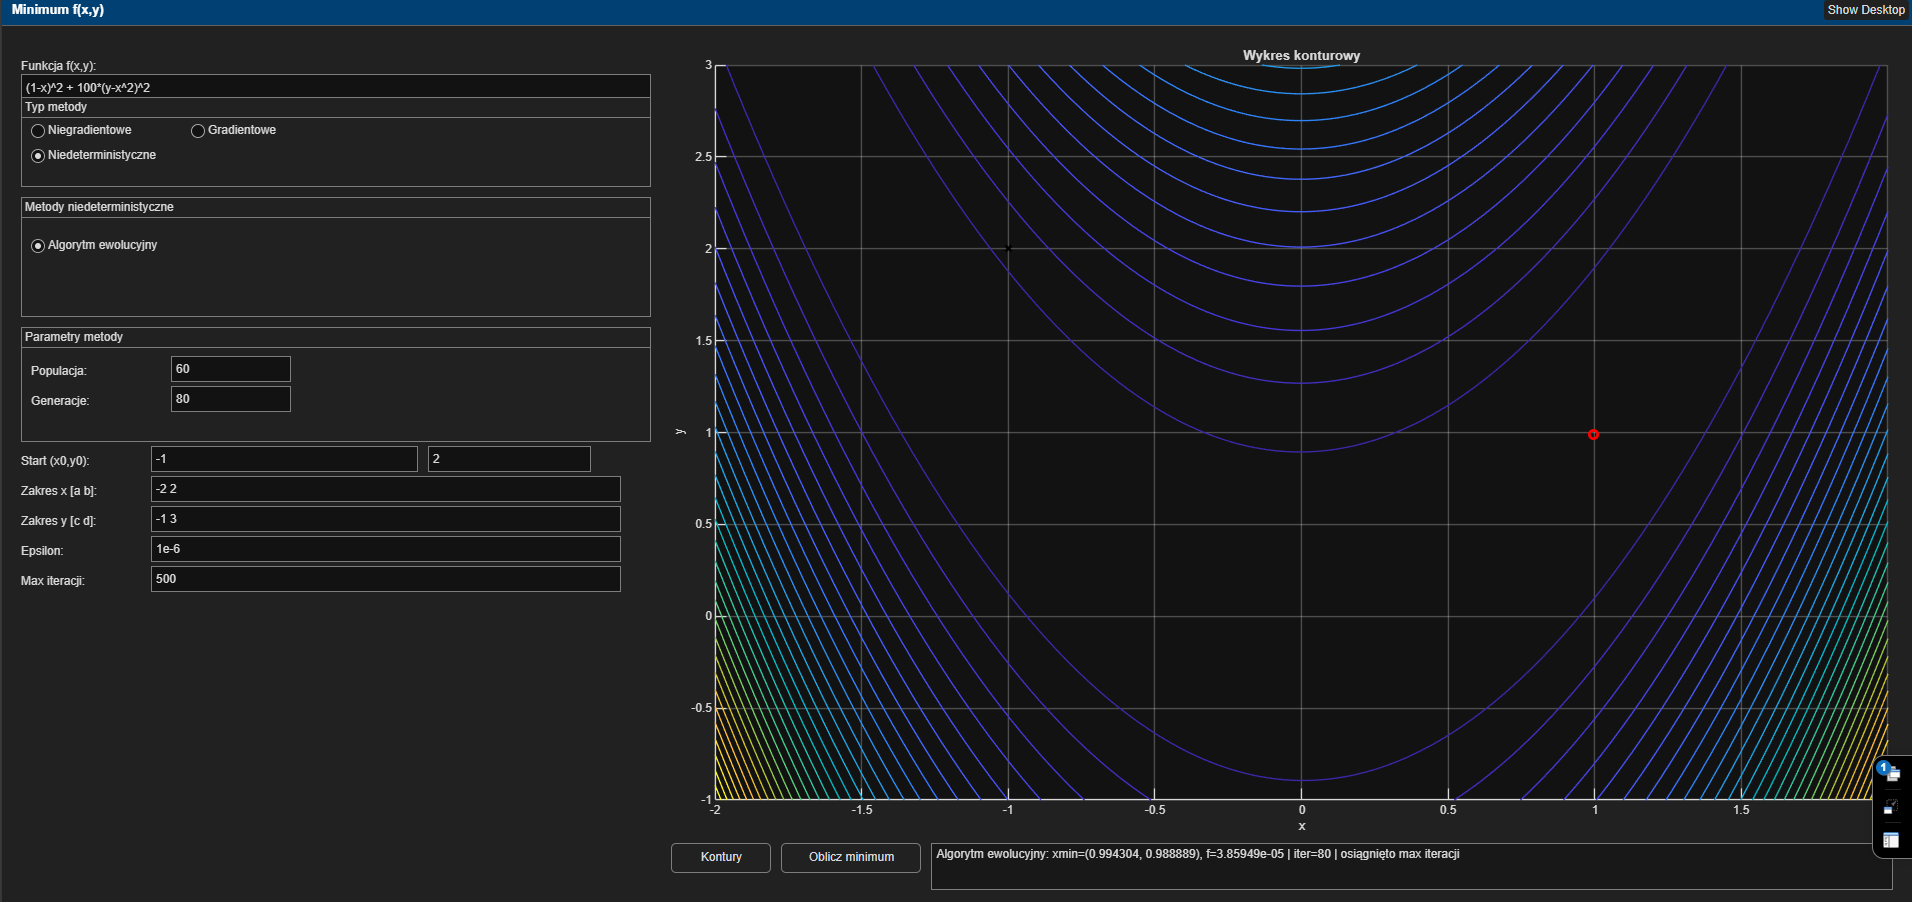
\includegraphics[width=1\textwidth]{figure/Figure1.png}
    \caption{Instrukcja obsługi}
\end{figure*}

Aplikacja służy do wyznaczania minimum funkcji dwóch zmiennych $f(x,y)$ z możliwością wyboru metody optymalizacji, ustawienia parametrów oraz wizualizacji wyniku na wykresie konturowym.

\subsubsection{Elementy interfejsu}

Interfejs składa się z następujących sekcji:

\begin{enumerate}
\item \textbf{Pole \emph{Funkcja f(x,y)}} – umożliwia wpisanie wzoru funkcji dwóch zmiennych w składni MATLAB.
Przykład:
\[
(1-x)^2 + 100\,(y-x^2)^2.
\]
Wzór musi być poprawnym wyrażeniem zależnym od zmiennych \texttt{x} oraz \texttt{y}.

\item \textbf{Sekcja \emph{Typ metody}} – wybór kategorii algorytmu:
\begin{itemize}
\item \emph{Niegradientowe},
\item \emph{Gradientowe},
\item \emph{Niedeterministyczne}.
\end{itemize}
Po zmianie kategorii wyświetla się odpowiednia lista metod, a pozostałe listy są ukrywane.

\item \textbf{Sekcja wyboru metody} – lista algorytmów dostępnych w danej kategorii:
\begin{itemize}
\item \textbf{Niegradientowe:} Hooke--Jeeves, Nelder--Mead, Powell,
\item \textbf{Gradientowe:} Fletcher--Reeves, DFP, BFGS,
\item \textbf{Niedeterministyczne:} Algorytm ewolucyjny (GA).
\end{itemize}

\item \textbf{Panel \emph{Parametry metody}} – pojawia się dynamicznie i zawiera tylko te parametry,
które są istotne dla wybranej metody, np.:
\begin{itemize}
\item Hooke--Jeeves: krok $\delta$,
\item Fletcher--Reeves: krok początkowy $\alpha$,
\item GA: rozmiar populacji oraz liczba generacji.
\end{itemize}
Jeżeli metoda nie wymaga dodatkowych parametrów, w panelu pojawia się komunikat o ich braku.

\item \textbf{Parametry ogólne} – wspólne dla wszystkich metod:
\begin{itemize}
\item \textbf{Start $(x_0,y_0)$} – punkt początkowy dla metod deterministycznych,
\item \textbf{Zakres $x\in[a,b]$ oraz $y\in[c,d]$} – przedziały wykorzystywane do rysowania konturów oraz
jako ograniczenia w algorytmie GA,
\item \textbf{Epsilon} – tolerancja zakończenia (dokładność),
\item \textbf{Max iteracji} – maksymalny limit liczby iteracji (dla GA odpowiada maksymalnej liczbie generacji).
\end{itemize}

\item \textbf{Wykres konturowy} – przedstawia poziomice funkcji $f(x,y)$ na zadanym zakresie.
Na wykresie oznaczane są:
\begin{itemize}
\item punkt startowy $(x_0,y_0)$ jako znak \texttt{x},
\item wyznaczone minimum jako punkt (czerwone kółko).
\end{itemize}

\item \textbf{Pole wyniku} – tekstowe podsumowanie obliczeń w formacie:
\[
\texttt{metoda: xmin=(\dots), f=\dots \;|\; iter=\dots \;|\; powód zakończenia}.
\]
Powód zakończenia informuje, czy algorytm zakończył pracę z powodu spełnienia tolerancji
czy przez osiągnięcie limitu iteracji.
\end{enumerate}

\subsubsection{Procedura użycia}

Zalecany przebieg pracy z aplikacją:

\begin{enumerate}
\item Wprowadź wzór funkcji w polu \textbf{Funkcja f(x,y)}.
\item Ustaw \textbf{zakresy} $x\in[a,b]$ oraz $y\in[c,d]$ zgodnie z obszarem zainteresowania.
\item (Opcjonalnie) Ustaw punkt startowy \textbf{$(x_0,y_0)$} dla metod deterministycznych.
\item Wybierz \textbf{Typ metody} (niegradientowa / gradientowa / niedeterministyczna).
\item Wybierz konkretną metodę z listy.
\item Jeśli panel \textbf{Parametry metody} wyświetli dodatkowe pola, uzupełnij je.
\item Ustaw \textbf{Epsilon} (dokładność) oraz \textbf{Max iteracji} (limit obliczeń).
\item Kliknij \textbf{Kontury}, aby zaktualizować wykres konturowy (jeśli zmieniono funkcję lub zakresy).
\item Kliknij \textbf{Oblicz minimum}, aby uruchomić wybraną metodę optymalizacji.
\item Odczytaj wynik w polu tekstowym oraz z wykresu (zaznaczone minimum).
\end{enumerate}

\subsubsection{Uwagi praktyczne}

\begin{itemize}
\item Dla funkcji o wielu minimach lokalnych wynik metod deterministycznych może zależeć od punktu startowego $(x_0,y_0)$.
W takim przypadku zaleca się testowanie różnych punktów startowych oraz porównanie z algorytmem GA.
\item Zwiększenie \textbf{Epsilon} przyspiesza obliczenia kosztem dokładności.
Zmniejszenie \textbf{Epsilon} poprawia dokładność, ale może zwiększyć liczbę iteracji.
\item Parametr \textbf{Max iteracji} zabezpiecza przed zbyt długim działaniem algorytmu w sytuacji braku zbieżności.
\item W GA większa \textbf{Populacja} oraz większa liczba \textbf{Generacji} zwykle zwiększają szansę znalezienia lepszego minimum,
kosztem czasu obliczeń.
\item Jeżeli wykres konturowy jest ``spłaszczony'' lub trudno interpretowalny, warto zmienić zakresy $[a,b]$ i $[c,d]$
tak, aby obejmowały interesujący obszar funkcji.
\end{itemize}

\end{document}